\documentclass[12pt,a4paper]{report}
% \usepackage[utf8]{inputenc}
% \usepackage[vietnam]{babel}
\usepackage[utf8]{vietnam}
\usepackage{amsmath}
\usepackage{amsfonts}
\usepackage{amssymb}
\usepackage{graphicx}
\usepackage{color}
\usepackage{framed}
\usepackage[left=2cm,right=2cm,top=2cm,bottom=2cm]{geometry}

\title{\framebox {
        \textcolor{TEcolor}{
            \Huge {    AP/College Physics 1    }
        }
    }    }
    
\author{\Large @arch-techs}
\date{2021}

\definecolor{TEcolor}{RGB}{0, 50, 50}

\usepackage{fancyhdr}

\pagestyle{fancy}
\fancyhf{}
\lhead{
\includegraphics[scale=0.2]{TE1}
\textcolor{TEcolor}{
\fontfamily{cmss}\selectfont
@arch-techs}
}
\rhead{\textcolor{TEcolor} {
	\fontfamily{cmss}\selectfont AP/College Physics 1
}}
\rfoot{
\fontfamily{cmss}\selectfont \textcolor{TEcolor}{
Page \thepage}}


\begin{document}
{\fontfamily{cmss}\selectfont
\begin{titlepage}
\maketitle
\end{titlepage}
\newpage

\begin{center}
    \begin{center}
    \framebox {
        \textcolor{TEcolor}{
            \Large {    AP/College Physics 1    }
        }
    }    
    \end{center}
    
    \vspace{5mm}
    
    by: @arch-techs
    
    \vspace{1cm}
    
    \begin{enumerate}
        \item Distance and displacement
            \begin{figure}[h]
                \centering
                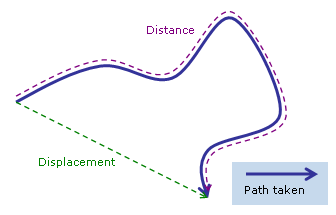
\includegraphics[scale=0.7]{Distancedisplacement}
                \fontfamily{cmss}\selectfont {
                    \caption{Distance and displacement}
                }
                \label{fig:my_label}
            \end{figure}
            \begin{itemize}
                \item Displacement: Change in position of an object. We use the symbol $\Delta x$ for displacement, where $\Delta$ means "change." A vector quantity with units of distance.
                \item Distance: Total amount the object has moved. This depends on the whole path traveled, not just the starting and ending points. Distance traveled is always a non-negative number. A scalar quantity with units of distance.
                \item Equation: \newline
                
                \begin{equation} \label{eu_eqn}
					\Delta x = x - x_{0}   		
         		\end{equation}
				\begin{center}
				$\Delta x$ is displacement, $x$ is the final position, $x_{0}$ is the initial position.
				\\
				Displacement is the difference between the final and initial positions.
				\end{center}				         		
         		
                
            \end{itemize}
            
   		\item Average velocity and speed
   			\begin{align*}
   				\overline{v} = \dfrac{\Delta x}{\Delta t} && / && v_{arg} = \dfrac{d}{\Delta t}
   			\end{align*}
   				
   		
            
    \end{enumerate}
    
\end{center}




}
\end{document}